\chapter{Theoretical Framework}
This chapter outlines the theoretical foundations and the specific tools and technologies employed in the
design, development, and implementation of a mobile application for fish species identification. The theoretical framework describes how such a system could leverage state-of-the-art machine learning techniques for
fish species classification and utilize modern software development frameworks and tools to build a robust
and user-friendly mobile application with a supporting backend system. The selection of each component is
guided by the need to create an effective, efficient, and adaptive system capable of performing fish identification in real-world conditions and improving over time.

\section{Foundation in Deep Learning and Computer Vision}
The core functionality of an application designed for identifying and classifying fish species from visual
data is fundamentally rooted in the principles and advancements within the fields of Deep Learning and
Computer Vision. These disciplines provide the necessary theoretical and algorithmic basis for enabling
machines to interpret and derive meaningful information from images, tasks traditionally performed by
human observation.

\subsection{Deep Learning (DL)}
Deep Learning, a powerful subset of Machine Learning, utilizes artificial neural networks characterized
by multiple hidden layers to learn complex patterns and representations directly from raw data. This
hierarchical learning approach allows models to automatically extract increasingly abstract features from
input data, such as visual patterns in images. Unlike traditional machine learning techniques that often rely
on manually engineered features, DL models, particularly Convolutional Neural Networks (CNNs), excel at
automatically learning spatial hierarchies of features, progressing from simple edges and textures in early
layers to more complex object parts and configurations in deeper layers. This capability makes deep learning
highly suitable for intricate visual analysis tasks, such as recognizing and classifying diverse fish species from
images (Li, 2022). The study acknowledges the significant advancements that deep learning techniques have
brought to automating tasks like species classification and identification, offering a powerful enhancement
over traditional manual methods, which are time-consuming, error-prone, and limited in scalability (Austen
and Author, 2016; Fouad and Author, 2013). The models used for object detection, such as the YOLO
series, are fundamentally built upon CNN architectures for feature extraction.

\subsubsection{Convolutional Neural Networks (CNNs)}
CNNs are the cornerstone of modern deep learning for image-based tasks. Their architecture is specifically designed to handle spatial information by using convolutional layers that scan small receptive fields across the image, pooling layers that reduce dimensionality, and fully connected layers that integrate the extracted features for final classification.
The general flow of a CNN is illustrated in Figure~\ref{fig: Convolutional Neural Network Layers for Image Classification}.

\begin{figure}[H]
    \centering
    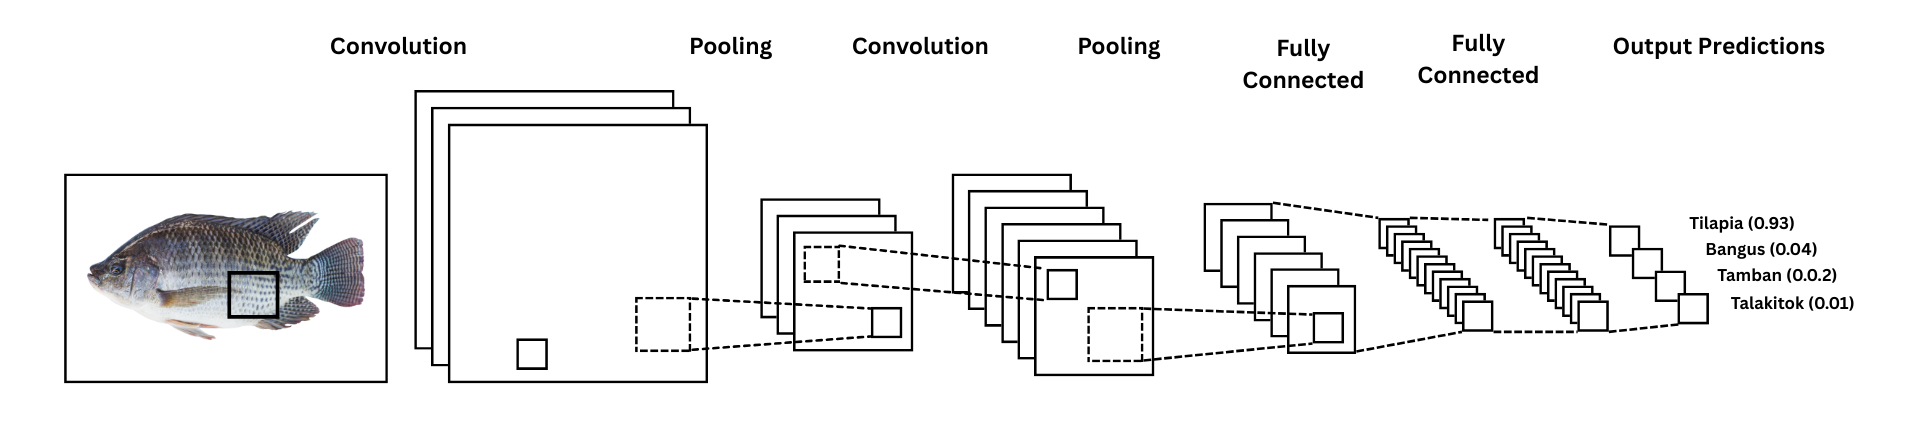
\includegraphics[width=1\textwidth]{images/images/Models/Convolutional Neural Network.png}
    \caption{Convolutional Neural Network Layers for Image Classification} 
    \label{fig: Convolutional Neural Network Layers for Image Classification}
\end{figure}


\subsection{Computer Vision}
Computer Vision is a field of artificial intelligence focused on enabling computers to interpret and understand
the world from digital images or videos. It encompasses a wide range of tasks, including image acquisition,
processing, object recognition, scene understanding, and visual data analysis. Deep learning has had a
transformative impact on Computer Vision, providing state-of-the-art algorithms that have significantly
advanced performance across many CV tasks compared to earlier methods based solely on handcrafted
features (Zou and Chen, 2023). Computer Vision is essential to a project of this nature as it provides the
overarching framework and specific techniques required for the system to ’see,’ process, and interpret the
fish images captured by a user’s smartphone to perform the task of identification.


\subsection{Object Detection: The Core Task}
While general image classification assigns a single label to an entire image, the specific visual analysis task
central to an application for fish identification is Object Detection. This capability is necessary because users’
images may contain multiple fish specimens, potentially of different species, within varying backgrounds.



\subsection{Definition of Object Detection}
Object Detection is a computer vision task that involves both identifying the presence of objects from a
predefined set of classes within an image and determining their precise location. This location is typically represented by a bounding box tightly enclosing each detected object instance. Object detection therefore
combines elements of image classification (assigning a class label) and object localization (determining spatial coordinates), differentiating it from image classification (single label for the whole image) or semantic
segmentation (pixel-level classification).

\subsubsection{Object Detection Architectures}
Modern deep learning-based object detection algorithms generally fall into two categories: two-stage detectors and single-stage detectors (Soviany and Ionescu, 2018; Zou and Chen, 2023). Two-stage methods
(e.g., Faster R-CNN) first propose regions of interest likely containing objects and then classify and refine
these proposals in a second stage. Single-stage methods (e.g., YOLO, SSD) bypass the region proposal
step, performing classification and bounding box regression directly across the entire image in a single pass.
While two-stage detectors can sometimes achieve marginally higher accuracy, single-stage detectors are significantly faster, making them the preferred approach for applications requiring real-time or near real-time
performance, such as mobile applications. This difference in processing strategy represents a key theoretical
trade-off between potential maximum accuracy and inference speed.

 \subsection{Ultralytics YOLO Framework}
Ultralytics YOLOv11 is a modular, production-ready object detection framework built on PyTorch. It offers streamlined capabilities for model training, evaluation, conversion (e.g., to TensorFlow Lite), and deployment. The framework supports rapid prototyping through YAML-based architecture definitions, automated logging, and built-in export tools for multiple formats including ONNX, TFLite, and CoreML—making it well-suited for real-time applications, particularly on mobile and embedded devices.

 \subsection{The YOLO (You Only Look Once) Algorithm (Specifically YOLOv11)}
Based on the principles of single-stage object detection, this theoretical framework considers the YOLO (You
Only Look Once) algorithm. The YOLO family is renowned for its high detection speed, which is crucial for
real-time applications, while maintaining competitive accuracy compared to other object detection paradigms
(Diwan and Author, 2023).
n
\subsection{Introduction to YOLO Series}
The fundamental theoretical premise of YOLO is to transform the task of object detection into a single
regression problem. An input image is divided into a grid, and each grid cell is responsible for predicting
bounding boxes and associated confidence scores, along with conditional class probabilities for objects whose
center falls within that cell. A single convolutional neural network processes the entire image in one forward
pass to generate these predictions. This unified approach distinguishes YOLO from multi-stage pipelines
and contributes to its speed advantage. Since the initial introduction of YOLO, the architecture has evolved
through numerous versions, each building upon the last to improve performance across various benchmarks
(Diwan and Author, 2023).

\subsection{ Rationale for an advanced YOLO version (e.g., YOLOv11)}
A system described herein might utilize a model like YOLOv11. The selection of such a model would be
grounded in its standing as a cutting-edge iteration within the YOLO series. According to recent benchmark
studies (Jegham et al., 2024), advanced YOLO versions demonstrate an excellent balance between detection
accuracy and computational efficiency. A particularly relevant finding from a comparative study cited in
the literature review (Sharma and Author, 2024), which evaluated YOLO versions 8-11 and Faster R-CNN,
highlighted that YOLOv11 achieved the lowest inference time among all tested models (13.5 ms). This
low inference time is a critical theoretical and practical advantage for a mobile application, as it directly
impacts the speed at which detection results can be provided to the user on device hardware, enabling a
responsive, near real-time experience. While other versions might offer slightly higher accuracy in some
benchmarks, the superior speed of models like YOLOv11 makes them a theoretically optimal choice when
considering the constraints and requirements of a mobile, real-time application. The model operates using
a single convolutional neural network (CNN) as its backbone for feature extraction, followed by detection
heads that predict bounding boxes and class probabilities.

\subsection{YOLOv11 Architecture}
According to Sulake (2025), YOLOv11 introduces several architectural innovations aimed at improving small object detection, spatial awareness, and computational efficiency while retaining real-time performance. Its architecture is organized into three main components: Backbone, Neck, and Head, supported by attention mechanisms, as shown in Figure~\ref{fig: YOLOv11 Architecture}.
\begin{figure}[H]
    \centering
    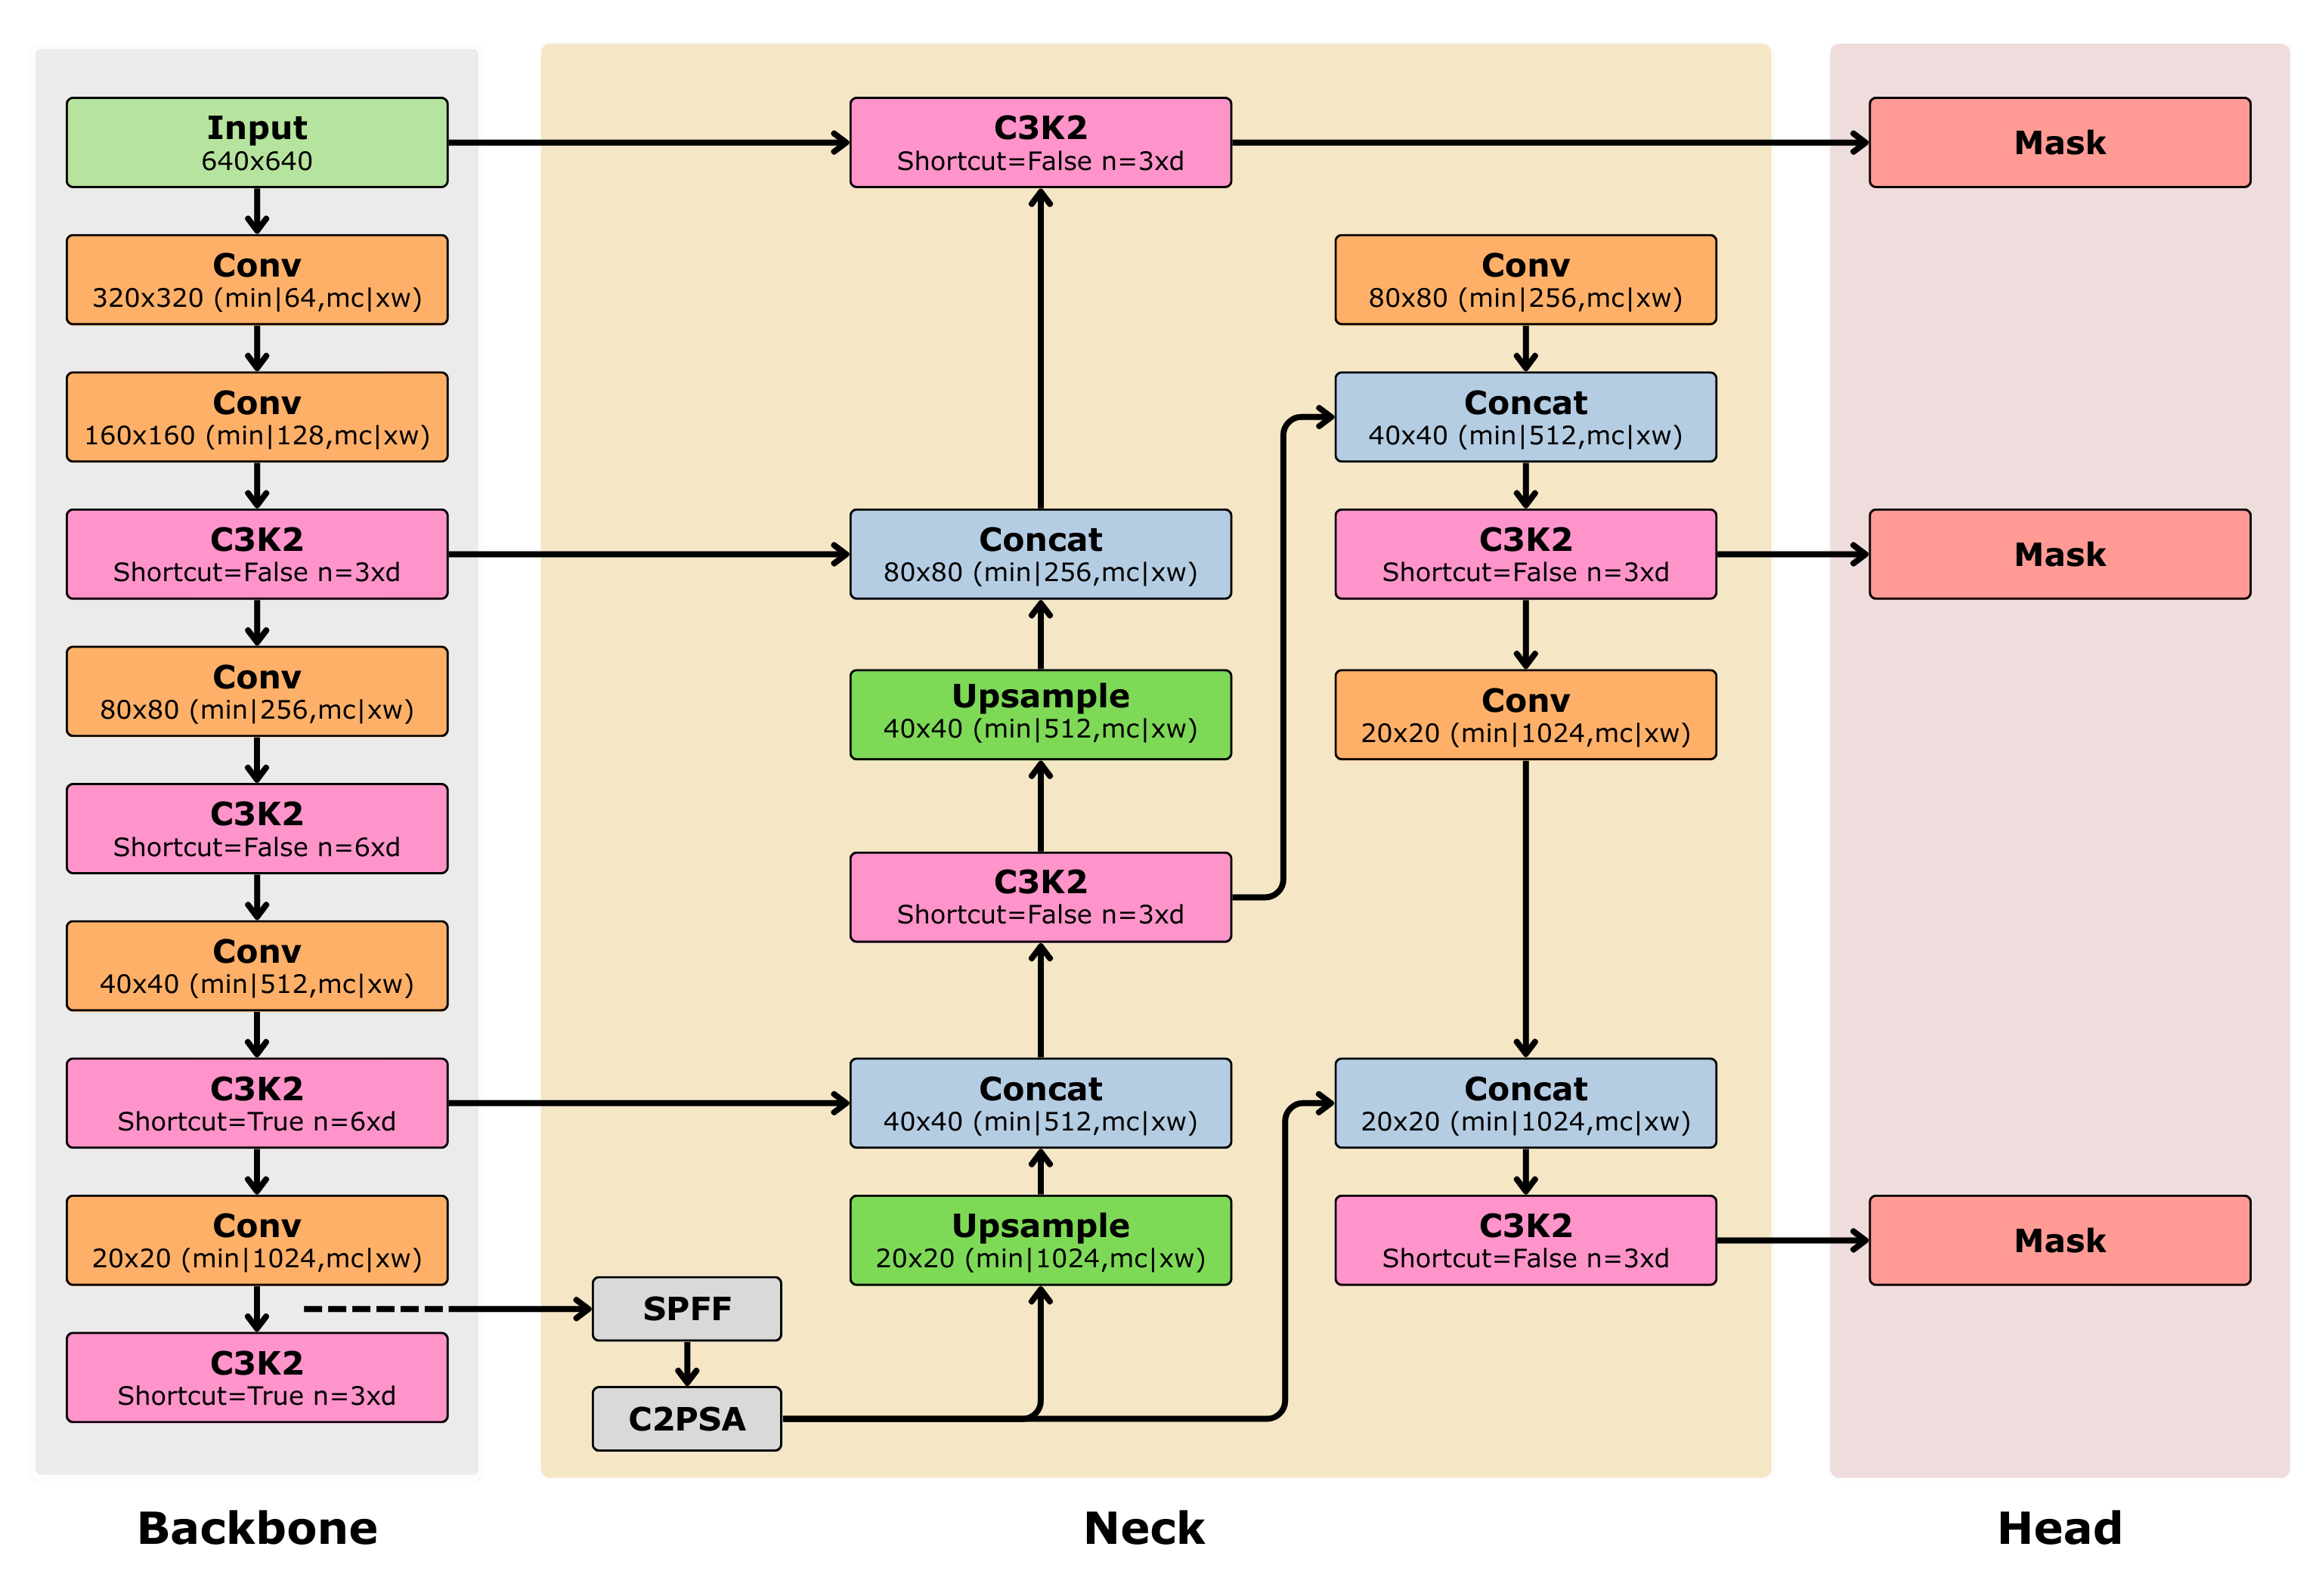
\includegraphics[width=0.9\textwidth]{images/images/Models/YOLOv11 Architecture.png}
    \caption{YOLOv11 Architecture} 
    \label{fig: YOLOv11 Architecture}
\end{figure}


The architecture can be summarized in the following components:
\begin{itemize}
\item\textbf{Backbone:}The backbone serves as the feature extractor, processing the input image to generate meaningful feature maps. YOLOv11 utilizes Convolutional Blocks (Conv Blocks) with Batch Normalization and SiLU activation, Bottleneck layers with optional residual connections, and the newly introduced C3K2 block. The C3K2 block employs smaller 3×3 kernels and a CSP-based structure to improve feature representation while reducing computational cost. This allows YOLOv11 to achieve a balance between detection accuracy and real-time performance.

\item\textbf{Neck (SPFF and Upsampling):} The Neck connects the Backbone to the detection layers. YOLOv11 adopts the Spatial Pyramid Pooling Fast (SPFF) module, which aggregates multi-scale features through parallel max-pooling operations of different kernel sizes. This enables the network to capture both global and local context, making it particularly effective in detecting small objects. Upsampling is also employed to fuse lower-level fine-grained features with higher-level semantic features.

\item\textbf{Attention Mechanism (C2PSA Block):} YOLOv11 incorporates the C2PSA (Cross Stage Partial with Spatial Attention) block, which applies position-sensitive attention to emphasize significant spatial regions within the feature maps. This mechanism allows the network to focus on small, occluded, or densely clustered objects, thereby improving detection robustness without introducing excessive computational overhead.

\item\textbf{Head (Detection Layer):} The detection head of YOLOv11 generates object predictions at multiple scales. It outputs bounding boxes, confidence scores, and class probabilities from three levels of feature maps (P3, P4, and P5). This multi-scale prediction design ensures that the model can detect small, medium, and large objects simultaneously.
\end{itemize}


\subsection{YOLOv11 Algorithm}
Sulake (2025) explains that YOLOv11 follows the one-stage detection paradigm but integrates new modules to improve accuracy, particularly for small and occluded objects. The algorithm can be described in the following steps:

\begin{itemize}
\item\textbf{Input Processing:} The input image is first resized to a fixed resolution and normalized to standardize pixel values. This preprocessing ensures consistency across inputs and reduces computational complexity while preserving essential visual features needed for detection.

\item\textbf{Feature Extraction (Backbone Stage):} The processed image is passed through the Backbone, which consists of Convolutional Blocks, Bottleneck layers, and the newly introduced C3K2 blocks. These modules work together to generate hierarchical feature maps that capture both low-level patterns (such as edges and textures) and high-level semantic information (such as object shapes and contexts).

\item\textbf{Multi-Scale Feature Aggregation (Neck Stage):} The extracted features are then processed by the Spatial Pyramid Pooling Fast (SPFF) module, which performs max-pooling at multiple scales to capture contextual information from different receptive fields. These features are combined with upsampled layers to strengthen the detection of objects across varying sizes, ensuring that both small and large objects are accurately represented in the feature maps.

\item\textbf{Attention-Based Refinement (C2PSA Stage):} The C2PSA block introduces spatial attention mechanisms that allow the network to focus on the most relevant regions of the image. By emphasizing critical features while suppressing less important ones, this stage significantly improves the detection of small, overlapping, or partially occluded objects.

\item\textbf{Multi-Scale Prediction (Head Stage):}The Detection Head generates predictions from three feature map levels (P3, P4, and P5), corresponding to small, medium, and large object scales. Each prediction includes bounding box coordinates, objectness scores (confidence that a box contains an object), and class probabilities (identifying the type of object). This multi-scale approach ensures accurate detection across a wide range of object sizes.

\item\textbf{Post-Processing (Non-Maximum Suppression):} Since multiple bounding boxes may overlap for the same object, YOLOv11 applies Non-Maximum Suppression (NMS) to eliminate redundant predictions. The algorithm retains only the bounding box with the highest confidence score while discarding others, ensuring that the final output contains precise and non-duplicated detections.

\item\textbf{Final Output:} After post-processing, the model produces the final detections in real time. Each detection includes the object’s class label, its confidence score, and the bounding box coordinates. This makes YOLOv11 suitable for real-time applications such as autonomous driving, video surveillance, and mobile object detection systems.
\end{itemize}



\section{Implementation Platform: Mobile and Backend Technologies}
To deliver the fish identification capability to users effectively, a robust implementation platform is required.
This involves developing a user-friendly mobile application and establishing a supporting backend infrastructure for data management, system logic, and model maintenance.

\subsection{Mobile Application (Front-end)}
A mobile application for fish identification would be designed to serve as an accessible and portable tool for
on-site fish identification, particularly relevant for users in environments like local wet markets. Smartphones
are ubiquitous and equipped with necessary hardware (camera, screen, processing) and user interface for
capturing images and receiving immediate identification feedback in real-world scenarios.


\subsection{Flutter Framework}
The mobile application could be developed using the Flutter framework. Flutter is an open-source UI
software development toolkit created by Google for building natively compiled applications for mobile, web,
and desktop from a single codebase. This cross-platform capability is a significant practical and theoretical
advantage, allowing the application to reach a wider audience on both Android and iOS devices without
the need for separate native development efforts, thereby enhancing development efficiency. Flutter provides
the framework for designing the user interface, integrating camera functionality, displaying the detection
results with bounding box overlays, presenting fish information, and enabling user interaction for feedback
submission.


\subsection{Model Integration with TensorFlow Lite and Ultralytics YOLO Flutter App}
To ensure the trained YOLO model runs efficiently on mobile device hardware with minimal latency and
reduced reliance on continuous internet connectivity, the model would be converted into TensorFlow Lite
format. TensorFlow Lite is a lightweight, mobile-optimized version of the TensorFlow machine learning
framework specifically designed for inference on edge devices. The integration of the TensorFlow Lite model
into the Flutter application could be facilitated by using frameworks like the Ultralytics YOLO Flutter
App framework, which provides the necessary tools and libraries to load and run Ultralytics YOLO models
within a Flutter environment. This setup allows the core object detection inference to occur directly on the
user’s device.


\subsection{SQLite Database (On-Device)}
For managing data locally on the mobile device, the application could utilize an SQLite database. SQLite is
a lightweight, serverless, file-based, transactional SQL database engine well-suited for resource-constrained
environments like mobile devices. Its primary role in such an application would be to provide local data
persistence for caching fish species information accessed by the user, storing a history of past detections,
and temporarily queuing user feedback data before synchronization with the backend server. This local
storage supports offline access to previously viewed information and ensures data is not lost immediately
upon collection. The Flutter application could interact with this database using a package like Drift.


\section{Backend System (Server-side)}
A backend system is essential to support functionalities that require centralized data management, processing,
user management, and system maintenance that are beyond the scope of the mobile device or require data
aggregation across users.

\subsection{Django Framework}
The backend server could be developed using the Django framework. Django is a high-level Python web
framework that promotes rapid development through its ”batteries included” approach and adheres to a
clean, pragmatic design philosophy. It is theoretically well-suited for building the necessary server-side
components for an application of this type, including the RESTful API and the web-based admin panel.
Django’s ORM (Object-Relational Mapper) facilitates interaction with the backend database, managing
models for users, fish species information, detection logs, feedback entries, and model metadata.


\subsection{RESTful API}
RESTful API endpoints would be designed and implemented using Django to serve as the communication
layer between the mobile application and the backend server. These APIs define a standardized way for the
mobile app to request and send data to the server, handling essential operations such as:

\begin{itemize}
\item{User authentication (login, registration) and profile management.}
\item{Submission of user feedback data.}
\item{Retrieval of comprehensive fish species information (nutritional, ecological, taxonomic, etc.) from the
central database.}
\item{Potential retrieval and download of updated machine learning models to the mobile device.}
\end{itemize}

\subsection{Backend Database (Centralized)}
While SQLite serves the mobile application, the Django backend would interact with a centralized database
system for managing data across all users and for persistent storage requiring server-side processing. This
database would store user account information, the authoritative source of detailed fish species data, all
submitted feedback entries (validated or unvalidated), detection logs synchronized from devices, and metadata related to the deployed ML models. This centralized repository is crucial for the admin review process,
aggregate data analysis, and serving information and model updates to mobile clients.

\newpage
\section{User Feedback Mechanism and Continuous Model Improvement}
A distinctive theoretical and functional aspect of such a system is the integrated user feedback mechanism.
This component is not merely a static feature but a dynamic process designed to create a self-improving
system by leveraging real-world user interactions to enhance the accuracy and robustness of the core AI
model over time.


\subsection{Theoretical Basis for Continuous Improvement}
The feedback system is conceptually grounded in the principles of Active Learning and the Human-inthe-Loop paradigm. In active learning, an algorithm interactively queries a user for labels on new data
points, typically those for which it is most uncertain or which are most informative for improving its performance. In a system for fish identification, users could act as annotators in the field, providing crucial ground
truth labels, particularly when the model’s prediction is incorrect. This mechanism addresses significant
challenges identified in the literature, such as the variability in fish appearance across different conditions
and the inherent limitations of a fixed training dataset (Rachmatullah and Supriana, 2018; Yang et al., 2020).
By systematically collecting and incorporating feedback on challenging or misclassified examples, the system
can learn from its errors and adapt to variations encountered in real-world deployment, making the model
more robust and accurate over time.


\subsection{Process and Validation Pipeline}
The user feedback process would be structured to ensure data quality for subsequent model retraining. After
the YOLO model provides a detection, the user could indicate if the prediction was correct or incorrect. If
incorrect, the user would be prompted to select the correct species from a list. This feedback data, including
the original image and associated metadata, would be submitted to the backend server via the RESTful API.
A critical theoretical and operational gatekeeper is the Admin Review process. System administrators
would access a web-based panel to review submitted feedback. Based on their expertise and consultation of
credible external references (academic publications, fisheries databases, etc.), administrators would validate
the user-provided correction. This manual validation step is theoretically important to filter out erroneous
user input and ensure that only high-quality, verified corrections are used to update the model, preventing
the propagation of potential user errors into the training data.
The overall flow of this feedback loop, from detection to user response, administrative validation, and eventual model retraining, is illustrated in Figure~\ref{fig: Process and Validation Pipeline}

\begin{figure}[H]
    \centering
    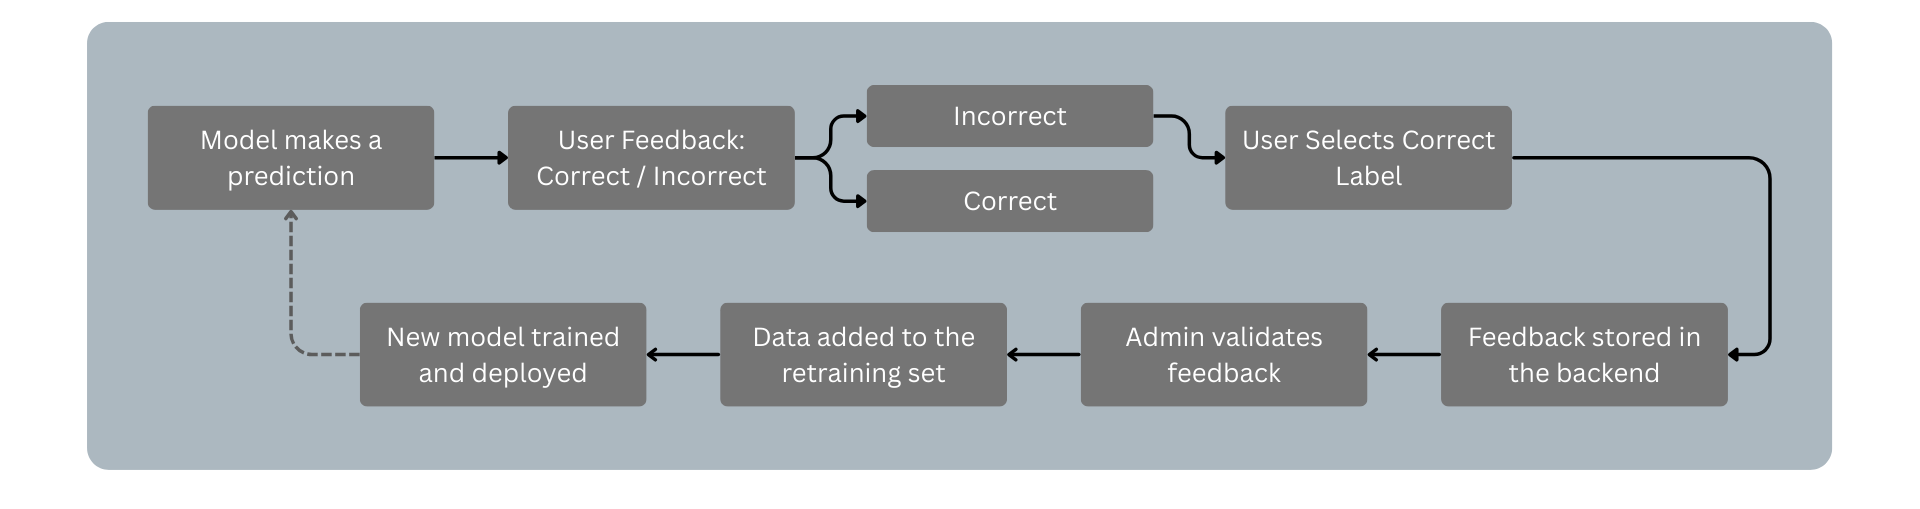
\includegraphics[width=1\textwidth]{images/images/Models/Process and Validation Pipeline.png}
    \caption{Process and Validation Pipeline} 
    \label{fig: Process and Validation Pipeline}
\end{figure}


\subsection{Model Retraining and Deployment Cycle}
Validated feedback entries would be stored in a dedicated repository, forming a valuable dataset of realworld cases where the model initially failed but the correct label is now known. A predefined Retraining Threshold would be applied uniformly across all fish species. This means that retraining would only be initiated manually once all 18 fish species have accumulated the required number of validated feedback entries. The YOLO model would then be fine-tuned or retrained using a combination of the original training dataset and this new, validated feedback data. The goal is to enable the model to learn from these specific challenging examples and improve its performance on similar instances in the future. After retraining is completed and the updated model’s performance is evaluated, it would be converted back to TensorFlow Lite format and deployed to the backend server. The mobile applications would be designed to check the server for updated models and download the latest version in the background, completing the feedback loop and ensuring that users benefit from the system’s continuous learning.

\subsection{Theoretical Impact}
This integrated feedback mechanism is not merely an added feature; it is a core component of the theoretical
framework that ensures the system’s long-term viability and increasing accuracy. It allows such a system
to adapt to real-world conditions, handle species variability, and overcome limitations inherent in the initial
training dataset (addressed by (Rachmatullah and Supriana, 2018) and the need for synthetic data or transfer
learning as mentioned by (Yang et al., 2020; Wan et al., 2021)). By incorporating user intelligence, the system
evolves, becoming more robust and reliable over time.


\section{Supporting Tools and Data Management Pipeline Components}
Beyond the primary ML framework and core development platforms, several supporting tools and pipeline
components are theoretically significant for enabling the development and operation of a system for fish
identification.

\subsection{Label Studio}
Label Studio could be used for the critical task of annotating the raw fish species image dataset. This
tool facilitates the manual drawing of bounding boxes around fish instances within images and assigning the
corresponding class labels. From a theoretical standpoint, this annotation process provides the necessary
labeled data for the supervised learning paradigm used to train the object detection model. The quality
and consistency of annotations directly impact the model’s ability to learn accurate object localization and
classification, making Label Studio an essential component in the data preparation phase of the ML pipeline.


\subsection{Figma}
Figma could be employed as the primary tool for the UI/UX design of the mobile application. It allows for
the creation of wireframes, mockups, and interactive prototypes. From a theoretical perspective related to
human-computer interaction and user-centered design, Figma facilitates the iterative design process aimed
at creating an intuitive and user-friendly interface. A well-designed interface is crucial for user engagement,
ease of image capture, clear presentation of results and information, and encouraging the submission of
valuable feedback, all of which are vital for the system’s success and the functioning of the feedback loop.


\subsection{Integration and System Synergy}
The theoretical framework for such a system is not merely a collection of individual concepts and technologies
but emphasizes the synergistic integration of these components to create a functional, efficient, and adaptive
system. The value proposition lies not in any single component but in the cohesive interaction of all parts.

